\chapter{Qué es una imagen para una computadora}
\label{cap:imagen}

\begin{enpocas}
Píxeles y canales de color, cómo forma una imagen una cámara, qué es el campo de visión, qué ve una
cámara que apunta hacia abajo, y por qué una persona a 30~m ocupa tan pocos píxeles.
\end{enpocas}

\section{Una imagen es una tabla de números}

La cámara del dron entrega imágenes de 1280 columnas por 960 filas: más de 1.2 millones de
\textbf{píxeles}. Cada píxel tiene tres números entre 0 y 255: cuánto rojo, cuánto verde y cuánto azul
(RGB). Una persona vista desde arriba es un pequeño grupo de píxeles de colores distintos al pasto: la
ropa, la piel, el cabello.

\begin{figure}[H]
\centering
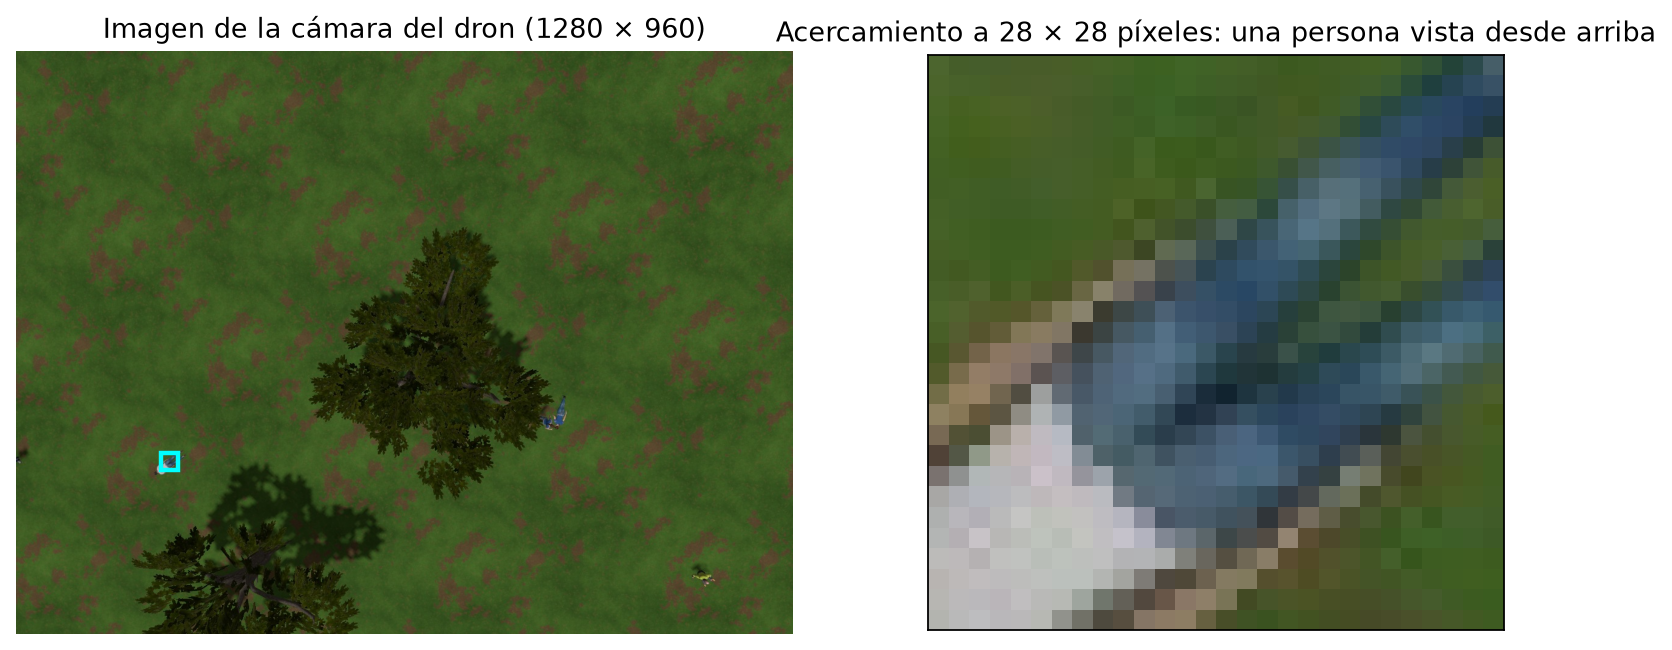
\includegraphics[width=\textwidth]{pixeles_persona.png}
\caption{Una imagen de la cámara del dron y un acercamiento a una de las personas: a 30~m, una persona
apenas ocupa unas decenas de píxeles.}
\end{figure}

\section{Cómo forma una imagen una cámara}

El modelo de \textbf{cámara estenopeica} supone una caja con un agujero: la luz de cada punto entra en
línea recta y llega a un punto del sensor. Un punto a distancia $Z$ y desplazado $X$ aparece en
\begin{equation}
u = f\,\frac{X}{Z},\qquad f = \frac{W/2}{\tan(\text{HFOV}/2)} = \frac{640}{\tan(0.87)} \approx 540\ \text{píxeles}.
\end{equation}
Toda la información de la cámara se resume en la \textbf{matriz intrínseca}
\begin{equation}
K = \begin{bmatrix} f & 0 & W/2\\ 0 & f & H/2\\ 0 & 0 & 1\end{bmatrix},
\end{equation}
que Gazebo publica en \cod{/camera_info}.

\begin{figure}[H]
\centering
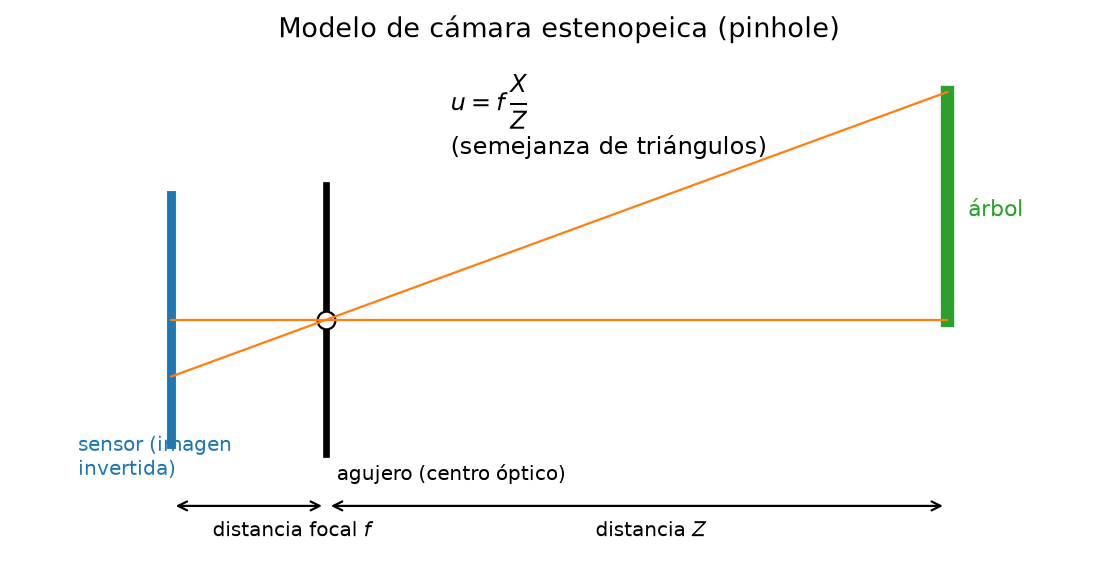
\includegraphics[width=0.8\textwidth]{c_estenopeica.png}
\caption{El modelo estenopeico: la imagen se forma por rayos rectos que pasan por el centro óptico.}
\end{figure}

\section{Una cámara que mira hacia abajo}

La cámara del Tarot 650 (la \cod{mono_cam} de PX4) tiene un campo horizontal de 1.74~rad (100°) y apunta al suelo. A 30~m de altura su
\textbf{huella} en el suelo mide
\begin{equation}
2\cdot30\cdot\tan(0.87) \approx 71\ \text{m}\ \text{de ancho}\quad\times\quad 53\ \text{m de alto}.
\end{equation}
Cada píxel cubre entonces unos $71/1280 \approx 5.5$~cm. Una persona de pie, vista desde arriba
(hombros de unos 45~cm), ocupa $\approx$8 píxeles de ancho; acostada, unos 30 de largo. Por eso hace
falta un detector entrenado para objetos pequeños y por eso la misión baja a 20~m para mirar mejor los
casos dudosos.

\begin{figure}[H]
\centering
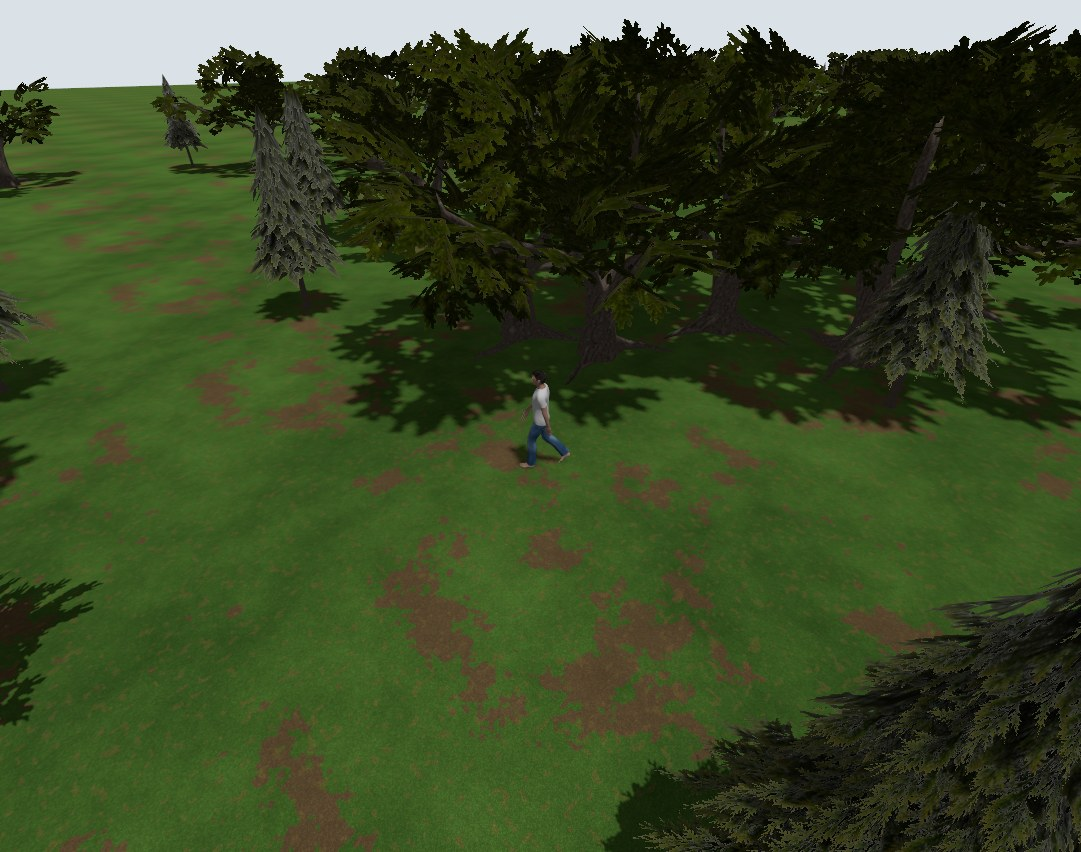
\includegraphics[width=0.49\textwidth]{gz_persona_de_pie.jpg}\hfill
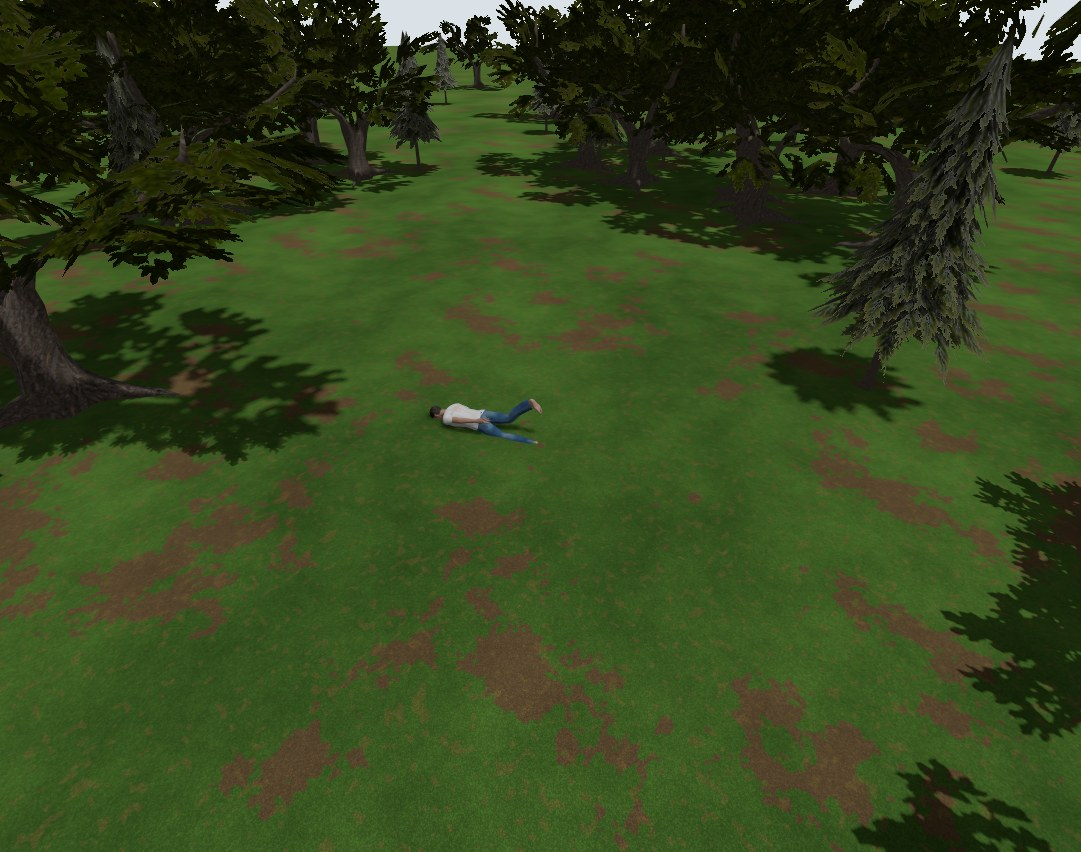
\includegraphics[width=0.49\textwidth]{gz_persona_acostada.jpg}
\caption{Una persona de pie y una acostada en el bosque simulado (vistas oblicuas para el libro; el
dron las ve desde arriba).}
\end{figure}

\section{Del píxel al mundo}

Un píxel no dice a qué distancia está lo que muestra, solo en qué \emph{dirección}: cada píxel es un
\textbf{rayo}. Para ubicar a la persona hay que cortar ese rayo con el suelo; si además se conoce la
incertidumbre de la posición y la orientación del dron, se puede calcular qué tan grande es el error
(capítulo~\ref{cap:localizacion}).

\begin{recuerda}
Una cámara da direcciones, no distancias. Con el suelo plano y la altura del dron, cada dirección se
convierte en un punto del mapa.
\end{recuerda}
